% Copyright 2021 Edoardo Riggio

% Licensed under the Apache License, Version 2.0 (the "License");
% you may not use this file except in compliance with the License.
% You may obtain a copy of the License at

% 	http://www.apache.org/licenses/LICENSE-2.0

% Unless required by applicable law or agreed to in writing, software
% distributed under the License is distributed on an "AS IS" BASIS,
% WITHOUT WARRANTIES OR CONDITIONS OF ANY KIND, either express or implied.
% See the License for the specific language governing permissions and
% limitations under the License.

\documentclass{article}

\usepackage{hyperref, amsmath, graphicx, amssymb}
\usepackage{fancyvrb, newverbs, xcolor, tikz}
\DeclareMathAlphabet{\mymathbb}{U}{BOONDOX-ds}{m}{n}

\usetikzlibrary{positioning}

\graphicspath{{./assets/}}
\definecolor{cverbbg}{gray}{0.93}

\newenvironment{cverbatim}
 {\SaveVerbatim{cverb}}
 {\endSaveVerbatim
  \flushleft\fboxrule=0pt\fboxsep=.5em
  \colorbox{cverbbg}{\BUseVerbatim{cverb}}%
  \endflushleft
}

\newenvironment{lcverbatim}
 {\SaveVerbatim{cverb}}
 {\endSaveVerbatim
  \flushleft\fboxrule=0pt\fboxsep=.5em
  \colorbox{cverbbg}{%
    \makebox[\dimexpr\linewidth-2\fboxsep][l]{\BUseVerbatim{cverb}}%
  }
  \endflushleft
}

\begin{document}
\begin{titlepage}
    \begin{center}
        \vspace*{1cm}
        
        \Huge
        \textbf{Quantum Computing Cheatsheet}
        
        \vspace{0.5cm}
        \LARGE
        
        \vspace{.5cm}
        
        Edoardo Riggio
   		  \vspace{1.5cm}
       
        \vfill
        
        \today
        
        \vspace{.8cm}
          \Large
          Quantum Computing - S.P. 2022 \\
        Computer Science\\
        Universit\`{a} della Svizzera Italiana, Lugano\\
        
    \end{center}
\end{titlepage}

\tableofcontents

\newpage

\section{What is Quantum Informatics}
\subsection{Information and Physics}
Experience, observation, and physical discourse are in the form of information. "It from Bit" -- John Wheeler \\ \\
Information representation, processing, and transmission are physical processes. "Information is physical" -- Rolf Landauer \\ \\
The representation of a bit must be physical. Moreover, digitalization comes very naturally with \textbf{quantization}. In classical physics, digitalization has to be enforced somehow (e.g., switched).

\subsection{Second Law of Thermodynamics}
The second law of thermodynamics states that, in a closed system, entropy does not increase. \\ \\
\textbf{Entropy} can be defined as a measure of disorder. Given $n$ binary memory cells containing random bits, if we erase all of the bits -- i.e., set them to 0 -- then the entropy in the set of memory cells drops.

\subsection{The Stern/Gerlach Experiment}
This experiment was proposed in 1921 by Otto Stern and later carried out in 1922 by Walther Gerlach. \\ \\
This is one of the most important experiments to understand the structure and properties of the basic building block of quantum information processing, the \textbf{Qbit}.

\begin{center}
	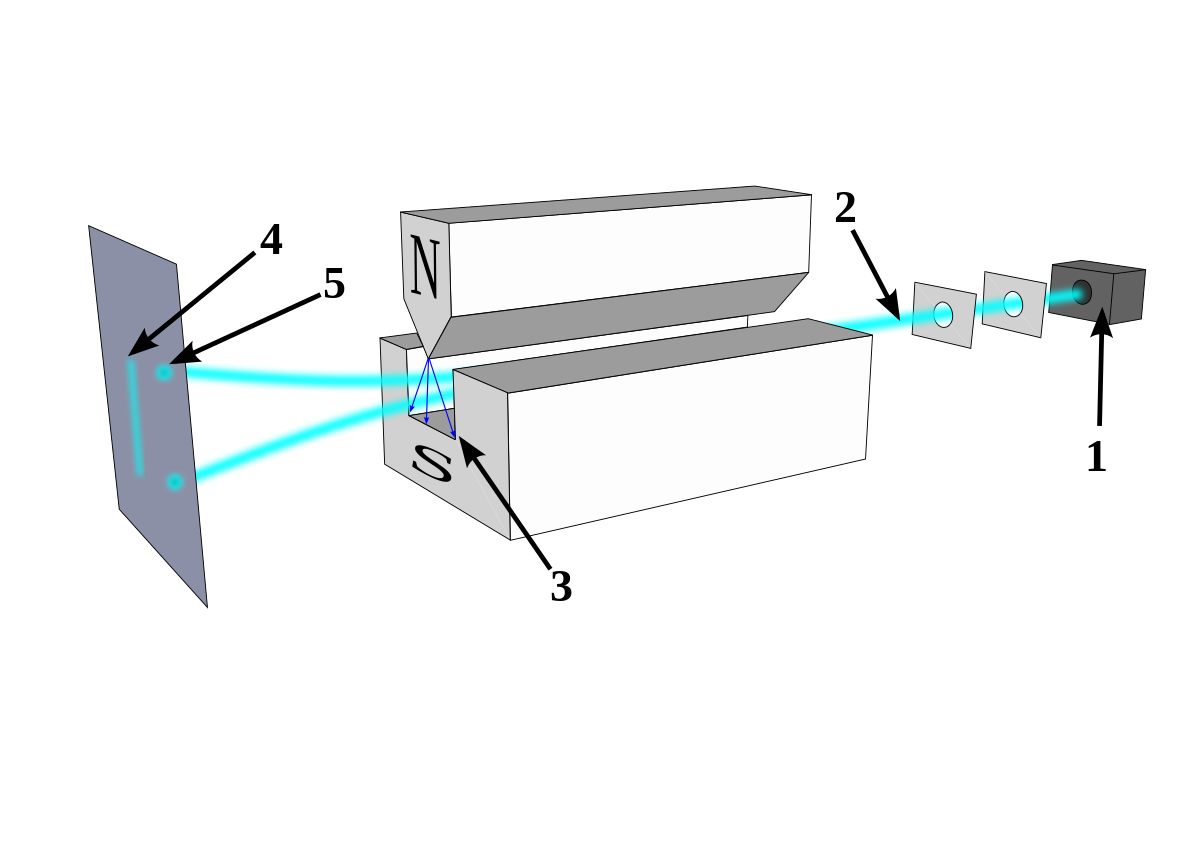
\includegraphics[width=8cm]{assets/stern_gerlach.png}
\end{center}
This experiment consisted of the measurement of the \textbf{magnetic dipole moment} of silver atoms. These silver atoms are sent as a stream (2) from an oven (1). Each atom is deflected from the path through an inhomogeneous magnetic field (3) and deflected from the path (5). This deflection is proportional to its dipole in the direction of the magnets. \\ \\
This experiment revealed no detection in the middle of the screen (4) but rather two sharp peaks at equal distances from the center (5). The quantity measured by the experiment is known in quantum mechanics as \textbf{spin}. \\ \\
In the case of a single measurement, for example, in the $z$-direction, it will result in two identical rays.

\begin{center}
	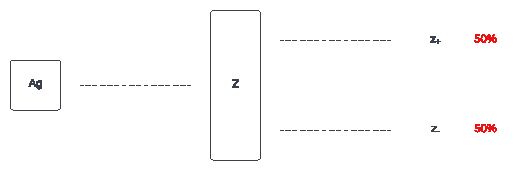
\includegraphics[width=10cm]{assets/one_z_measurement.pdf}
\end{center}
If the exact measurement is repeated for only one of the rays -- say $z_+$, then all the atoms are deflected again in the $+$ direction.

\begin{center}
	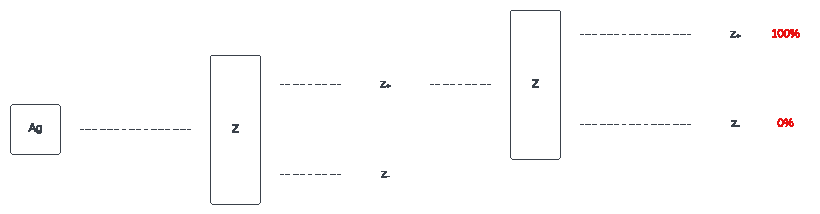
\includegraphics[width=11.5cm]{assets/two_z_measurements.pdf}
\end{center}
Finally, if the magnet is rotated and a $x$-direction measurement of the $z_+$ ray is made, another $z$-direction measurement, a 50-50 distribution. This puts the stability and the independence of the properties in question.

\begin{center}
	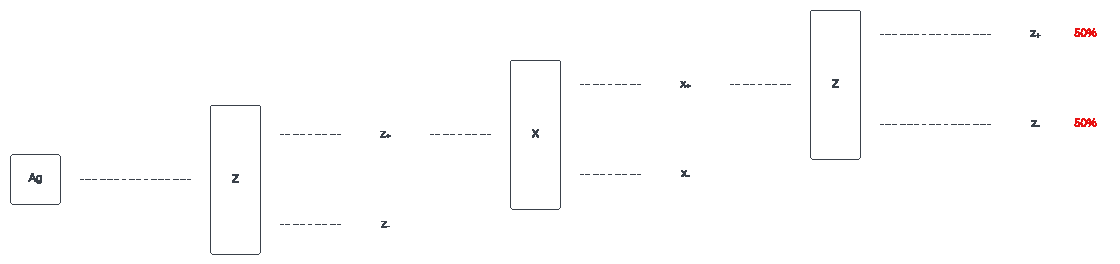
\includegraphics[width=12cm]{assets/z_x_z_measurements.pdf}
\end{center}

\subsection{Superposition}
Quantum superposition is a fundamental principle of quantum mechanics. It states that any two -- or more -- quantum states can be added together, and the result will be another valid quantum state. \\ \\
The question of whether a silver atom is in the state $| z_- \rangle$ or in the state $| z_+ \rangle$ are complementary to one another. They can be regarded as two answers to the same question -- i.e., the $Z$ measurement. \\ \\
If after performing an $X$ measurement, we want to know whether the silver atom is in a state $| x_+ \rangle$ or $| x_- \rangle$. Both are qual superpositions
\[ |x_+\rangle = \frac{1}{\sqrt{2}}|z_+\rangle + \frac{1}{\sqrt{2}}|z_-\rangle \]
\[ |x_-\rangle = \frac{1}{\sqrt{2}}|z_+\rangle - \frac{1}{\sqrt{2}}|z_-\rangle \]
No matter if we obtain one measurement or the other in the $Z$ measurement, the $X$-measurement either $| x_+ \rangle$ or $| x_- \rangle$ with equal probability. This is also known as a \textbf{quantum jump}.

\begin{center}
	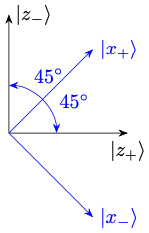
\includegraphics[width=2cm]{quantum_jump.png}
\end{center}

\subsection{Quantum Key Distribution}
We have seen that we can measure with certainty the same value in two consecutive measurements with the same basis. In other words, the interactions of a system with its environment become traceable. This traceability enables us to detect an eavesdropper in a \textbf{quantum cryptographic key agreement protocol}. \\ \\
The key distribution starts with \textit{Alice} using random measurements to encrypt the data. The encrypted photons are then sent to \textit{Bob}, which also uses random measurements to try and decrypt the data. After this process has terminated, \textit{Alice} sends the measurement basis she used to \textit{Bob} on a public channel. \textit{Bob} now takes the measurement basis and confronts it with his basis. The equal measurements are used as the \textbf{key}. \\ \\
If an eavesdropper, say \textit{Eve}, tries to intercept the message, she will need to guess the measurements for each photon. If the measurement is wrong, the system is disturbed. This means that \textit{Eve} has a probability of $1/4$ to be wrong in each stage. Thus, there is an almost 100\% probability of whether there was an eavesdropper.

\subsection{The Double-Slit Experiment}
If one shines a light onto a double slit, an interference pattern appears on the screen behind the double slit.

\begin{center}
	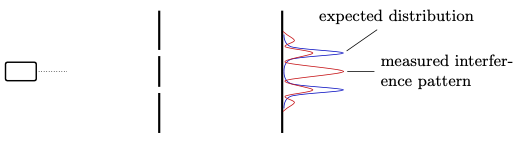
\includegraphics[width=10cm]{assets/double_slit.png}
\end{center}
If we were to measure the position of the photons on the screen (to the right of the image), an interference pattern would emerge. This means that single particles exhibit wave properties. However, the interference pattern disappears if we look at the particles' paths.

\subsection{The Mach/Zehnder Interferometer}
The Mach/Zehnder interferometer can be considered a variant of the double-slit experiment.

\begin{center}
	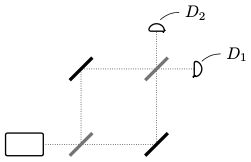
\includegraphics[width=5cm]{assets/interferometer.png}
\end{center}
If one sends single photons into the interferometer, the interference will occur, and the photons will be detected with certainty in detector $D_1$. \\ \\
In each \textbf{reflection}, the photon will pick up a phase shift of $\pi / 2$. Let us label the state of the photon moving to the \textbf{right} as $|1\rangle$, and the state of the photon moving \textbf{up} as $|2\rangle$. Their effect on \textbf{fully-reflecting mirrors} will then be:
\[ |1\rangle \mapsto i|2\rangle ~~~~~~~~ |2\rangle \mapsto i|1\rangle \]
While the effect on \textbf{semi-transparent mirrors} is:
\[ |1\rangle \mapsto \frac{1}{\sqrt{2}}(|1\rangle + i|2\rangle) ~~~~~~~~ |2\rangle \mapsto \frac{1}{\sqrt{2}}(|2\rangle + i|1\rangle) \]
Since we have these linear mappings, we can now track the photon through the interferometer. Since the emitter sends it to its right, the photon will start with a state of $|1\rangle$ --. Then we will have the following when hitting the \textbf{first semi-transparent mirror}:
\[ |1\rangle \mapsto \frac{1}{\sqrt{2}}(|1\rangle + i|2\rangle) \]
Now, the photon encounters a \textbf{fully-reflective mirror}, thus we need to apply the mappings to both $|1\rangle$ and $|2\rangle$ of the previous mapping:
\[ \frac{1}{\sqrt{2}}(|1\rangle + i|2\rangle) \mapsto \frac{1}{\sqrt{2}}(i|2\rangle + i \cdot i|1\rangle) \mapsto \frac{1}{\sqrt{2}}(i|2\rangle - |1\rangle) \]
Finally, the photon will again encounter a \textbf{semi-transparent mirror}. Thus, we will need to apply the mappings to both $|1\rangle$ and $|2\rangle$ again.
\begin{align*}
	\frac{1}{\sqrt{2}}(i|2\rangle - |1\rangle) &\mapsto \frac{1}{\sqrt{2}}\left(i\frac{1}{\sqrt{2}}(|2\rangle + i|1\rangle) - \frac{1}{\sqrt{2}}(|1\rangle + i|2\rangle) \right) \\
	&\mapsto \frac{1}{\sqrt{2}} \left( \frac{1}{\sqrt{2}}(i|2\rangle + i \cdot i|1\rangle) - \frac{1}{\sqrt{2}}(|1\rangle + i|2\rangle) \right) \\
	&\mapsto \frac{1}{\sqrt{2}} \left( \frac{1}{\sqrt{2}}(i|2\rangle - |1\rangle) - \frac{1}{\sqrt{2}}(|1\rangle + i|2\rangle) \right) \\
	&= -|1\rangle
\end{align*}
The photon, which now has state $-|1\rangle$, will be measured with certainty by detector D1.

\subsection{Quantum Bit}
To transfer a bit into the quantum world, we associate 0 and 1 with two orthogonal vectors:
\[ |0\rangle = \begin{pmatrix} 1 \\ 0 \end{pmatrix} ~~~~~~~~ |1\rangle = \begin{pmatrix} 0 \\ 1 \end{pmatrix} \]
A general quantum state can now be written as a superposition:
\[ |\psi\rangle = \alpha |0\rangle + \beta |1\rangle ~~~~~~~\text{with}~\alpha, \beta \in \mathbb{C};~\text{and}~|\alpha|^2 + |\beta|^2 = 1 \]
Measuring $|\psi\rangle$ in the standard basis will yield:

\begin{itemize}
	\item 0 -- With a probability of $|\alpha|^2$
	\item 1 -- With a probability of $|\beta|^2$
\end{itemize}

\subsubsection{Hadamard Gate}
Quantum circuits are composed of quantum gates which are \textbf{unitary maps}. The most important gate is the Hadamard gate. Which can be formalized as follows:
\[ H = \frac{1}{\sqrt{2}} \begin{pmatrix} 1 & 1 \\ 1 & -1 \end{pmatrix} \]
Which maps to the following superpositions:
\[ H|0\rangle = \frac{1}{\sqrt{2}}(|0\rangle + |1\rangle) ~~~~~~~~ H|1\rangle = \frac{1}{\sqrt{2}}(|0\rangle - |1\rangle) \]
Applying the Hadamard gate again will yield the standard basis vectors again.

\subsubsection{Square Root of NOT}
Another interesting gate is the following:
\[ F = \frac{1}{\sqrt{2i}} \begin{pmatrix} 1 & i \\ i & 1 \end{pmatrix} \]
When we apply this gate twice, we will obtain:
\[ F \cdot F = \begin{pmatrix} 0 & 1 \\ 1 & 0 \end{pmatrix} \]
In classical mechanics, no gate yields the not-gate this way. The gate $F$ has thus been called the "square root of NOT".

\subsection{Deutsch's Algorithm}
Given a function
\[ f : \{ 0, 1 \} \rightarrow \{ 0, 1 \} \]
We want to find out whether $f$ is constant and $f(0) \oplus f(1)$ is 0 or 1. We would have to query the function twice in classical mechanics to get both answers. But there is another way to find out. First, we must transform the black box into a \textbf{quantum black box}. Because of the unitarity of the quantum mechanical time evolution, the quantum box is \textbf{reversible}.

\begin{center}
	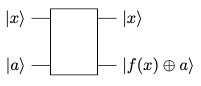
\includegraphics[width=4cm]{assets/deutsch.png}
\end{center}
This means that, if $a$ is 0, then $x$ is mapped to $|f(x)\rangle$ on the ouput wire. Moreover, if $a$ is 1, then $x$ is mapped to $\overline{|f(x)\rangle}$ -- which is the negation of $|f(x)\rangle$. \\ \\
If we were to put a superposition on the input wire and set $a$ to 0, we would obtain the following combined input:
\[ \frac{1}{\sqrt{2}}(|0\rangle + |1\rangle) \otimes |0\rangle = \frac{1}{\sqrt{2}} (|0\rangle \otimes |0\rangle + |1\rangle \otimes |0\rangle) \]
If:
\[ |0\rangle \otimes |0\rangle \mapsto |0\rangle \oplus |f(0)\rangle ~~~~~~~~ |1\rangle \otimes |0\rangle \mapsto |1\rangle \oplus |f(1)\rangle \]
Then, by linearly combining the two we obtain:
\[ \frac{1}{\sqrt{2}}(|0\rangle + |1\rangle) \otimes |0\rangle \mapsto \frac{1}{\sqrt{2}}(|0\rangle \oplus |f(0)\rangle + |1\rangle \oplus |f(1)\rangle \]
The resulting state is said to be \textbf{entangled}. This means that we cannot access information about $f(0)$ and $f(1)$ by merely measuring the output wire. However, if we also put a superposition on the second wire
\[ |a\rangle = \frac{1}{\sqrt{2}}(|0\rangle - |1\rangle) \]
Then we can expand the combined input as:
\begin{align*}
	& \frac{1}{\sqrt{2}}(|0\rangle + |1\rangle) \otimes \frac{1}{\sqrt{2}}(|0\rangle - |1\rangle) \\
	=~& \frac{1}{\sqrt{2}}(|0\rangle \otimes |0\rangle - |0\rangle \otimes |1\rangle + |1\rangle \otimes |0\rangle  - |1\rangle \otimes |1\rangle)
\end{align*}
Applying the gate to each summand, we obtain:
\[ \frac{1}{\sqrt{2}} \left( |0\rangle \otimes \big( |f(0)\rangle - \overline{|f(0)\rangle} \big) + |1\rangle \otimes \big( |f(1)\rangle - \overline{|f(1)\rangle} \big) \right) \]
If $f(0) = f(1)$, then:
\[ \frac{1}{\sqrt{2}}(|0\rangle + |1\rangle) \otimes \big( |f(0)\rangle - \overline{|f(0)\rangle} \big) \]
Otherwise:
\[ \pm \frac{1}{\sqrt{2}}(|0\rangle - |1\rangle) \otimes \big( |f(0)\rangle - \overline{|f(0)\rangle} \big) \]
If we now measure the standard basis of the output -- after having applied the Hadamard gate, this will yield:

\begin{center}
	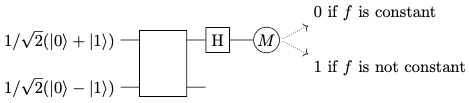
\includegraphics[width=9cm]{assets/deutsch2.png}
\end{center}
This algorithm does not allow us to retrieve more information. It does not yield the values of $f(0)$ or $f(1)$. What it yields is the result of $f(0) \oplus f(1)$.

\subsection{The Aspect/Gisin/Zelinger Experiments}
Quantum information processing is more than the fact that "a pair of Qbits is just one Qbit plus another Qbit". A striking manifestation is that other qualities arise when two entangled Qbits are independently measured. \\ \\
Imagine that -- inside of a preparation center -- pairs of Qbits (i.e., polarized photons) are generated and sent onto their respective paths to two parties -- \textit{Alice} and \textit{Bob}. What is sent to both \textit{Alice} and \textit{Bob} are two parts of the equal superpositions of $|0\rangle \otimes |0\rangle$ and $|1\rangle \otimes |1\rangle$. If \textit{Alice} and \textit{Bob} both measure in the standard basis -- i.e., $\{ |0\rangle, |1\rangle \}$, then they always receive the same output: a \textbf{perfect correlation}.

\subsubsection{Einstein/Podolsky/Rosen's Claim}
These three scientists, in 1935, claimed that quantum theory was \textbf{incomplete} and that it must be augmented by some "hidden parameters" that determine the measurement outcomes of all alternative measurements entirely.

\subsubsection{Bell's Claim}
Bell gave \textit{Alice} and \textit{Bob} more freedom. Now they could do measurements on a standard basis and other orthogonal bases. Bell claimed that EPR (Einstein/Podolsky/Rosen) is in doubt. There exist quantum correlations that go beyond the explanatory power of shared classical information. To prove it, Bell used a \textbf{singlet} and made \textit{Alice} and \textit{Bob} make measurements on different bases. \\ \\
Moreover, Bell discovered that measurement results are correlated; however, this correlation arises only upon measurement -- and not before it. This is known as \textbf{Bell non-locality}.

\section{Information is Physical}
A computing device essentially transforms \textbf{electrical free energy} into \textbf{heat}. If we consider a Turing Machine, even for deterministic TMs, computations are not logically reversible.

\subsection{Thermodynamics and Entropy}
\subsubsection{First Law}
The first law of thermodynamics says that the total energy is constant in a closed system. Moreover, a perpetuum mobile of the first kind is impossible.

\subsubsection{Second Law}
The second law of thermodynamics says that in a closed system, entropy does not decrease. Moreover, a perpetuum mobile of the second kind is impossible. \\ \\
This law is \textbf{asymmetric in time}.

\subsection{Information Theory}
Information theory was developed in 1948 by Claude Shannon to determine the fundamental limits of signal-processing operations such as \textbf{data compression on reliable storage} and \textbf{communication}.

\subsubsection{Standard Model of Communication}
Information theory initially focused on communication. In the most common scenario, we have \textit{Alice} and \textit{Bob} sending information to one another.

\begin{center}
	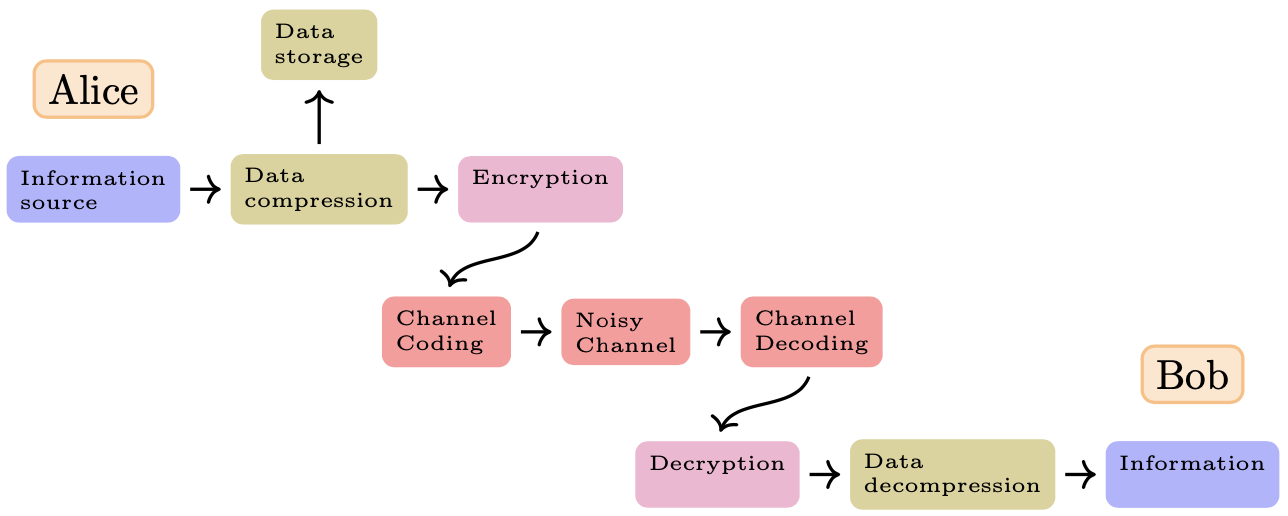
\includegraphics[width=12cm]{assets/information_theory.png}
\end{center}
A model usually contains \textbf{compression} to reduce the size of the data representing specific information. \textbf{Encryption} is then used to minimize attacks upon information transfer. \textbf{Channel coding} is used to introduce redundancy to protect against errors during transmission. Finally, there are all of the counterparts of the previous steps.

\subsubsection{The Game of 20 Questions}
If we imagine that \textit{Bob} can retrieve a secret by \textit{Alice} just by using 20 yes/no questions. \\ \\
Since \textit{Bob} from 20 questions can receive 20 answers -- 20 bits, this means that he will be able to distinguish between $2^20$ different questions. \\ \\
Assuming that \textit{Alice} chooses an element $x \in X$. \textit{Bob} now wants to determine which element \textit{Alice} has chosen. To do so, one could divide the set $X$ into subsets of equal size and ask in which one the chosen element was. The number of questions now is:
\[ \#Q = \lceil \log_2 |X|\rceil \]
This consideration motivated Hartley's formula for the \textbf{entropy of a uniform random variable X} over X (the elements), with
\[ P_x(x) = \frac{1}{|X|} \]
And the formula is:
\[ H(X) = \log_2|X| \]
Where the first $X$ is the random variable. Now, \textbf{uncertainty becomes a function of a random variable}. \textit{Bob}'s prior knowledge about \textit{Alice}'s choice can be formally described by a pdf (probability density function). For a general random variable, the measure of uncertainty -- i.e., the \textbf{entropy}, should correspond to the expectation value of the number of yes/no questions to find an element $x \in X$ using an optimal strategy and combining asymptotically many realizations of the random variable $X$.

\subsection{Entropy}
The entropy of a random variable $X$ over $X$, with distribution:
\[ P_X(x) = p_x \]
Is given by:
\[ H(X) = E[-(\log_2 P_X(x)] = - \sum_{x \in X} p_x \log_2p_x \]
In the case of a uniform distribution, the \textbf{entropy} of a random variable is equal to the size of its range. The \textbf{entropy of a macrostate} is the logarithm of the number of microstates that correspond to it. \\ \\
The \textbf{microstate} of a physical system specifies the position and momentum of each of the molecules. The \textbf{macrostate} of a physical system is a set of microstates.
\begin{center}
	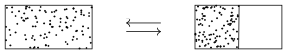
\includegraphics[width=5cm]{assets/entropy.png}
\end{center}
In the example above, the probability of going from the state on the left to the state on the right is:
\[ 2^{-N} \]
Where $N$ is the \textbf{number of particles}. Moreover, the entropy difference is:
\[ \Delta S = -Nk \ln 2 \]
Where $N$ is the \textbf{number of particles} and $k$ is the \textbf{Boltzmann's constant}. We can say that the right-to-left transition is \textbf{probable}, and allows for \textbf{gaining work}. \\ \\
The left-to-right transition can be enforced. For instance, this can be done by pushing a piston. Although in this case, the gas will cease to be in a closed system. 
\begin{center}
	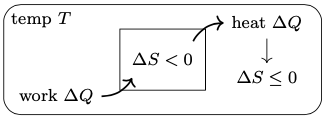
\includegraphics[width=5cm]{assets/piston.png}
\end{center}
In this case, the amount of entropy in the gas decreases. To compress this gas, we will have to use a certain amount of \textbf{free energy}. This energy will then be dissipated into the environment as \textbf{heat}. \\ \\
The minimal investment in terms of free energy to enforce that entropy decreases is:
\[ \Delta Q \geq \Delta S \cdot T \]

\subsection{Bit Analogy}
If we interpret the molecule in the canister as storing one bit -- a 0 if it is on the left and a 1 if it is on the right, forcing the molecule to the left would correspond to erasing that bit. \\ \\
The price for erasing that bit is:
\[ kT \ln 2 \]
This, together with the claim that it's irrelevant by what physical system the bit is stored, is called \textbf{Landauer's Principle}.

\subsection{Landauer's Principle}
Erasing a bit requires
\[ kT \ln 2 ~~~ (\approx 3 \times 10^{-21} J~ \text{at room tempterature}) \]
Of free energy. This energy must, in the process, be dissipated into the environment.

\subsection{The Converse of Landauer's Principle}
The inverse process of erasure, which is \textbf{randomization}, allows for the gain of free energy. For example, the amount of environmental heat energy that can be transformed into work is $kTN\ln2$ -- in the case of an \textit{all-0-string} of length $N$. Another example is the string of the first $N$ digits of the decimal expansion of $\pi$, which is $kTN\log10$. \\ \\
The previously defined examples offer the possibility of a logically reversible computation between the given string (for example, the first N decimal digits of $\pi$) and the \textit{all-0-string} of the same length.

\subsection{Bennett's Solution to Maxwell's Demon}
The demon must erase all the information accumulated in its brain during the sorting procedure. The necessary heat dissipation will exactly compensate for the entropy decrease. The demon must have an internal state depending on its observations and guiding its actions. \\ \\
This does not violate the second law of thermodynamics, as the demon will generate heat whenever it resets its internal memory to a known state. This will result in an entropy decrease and the emission of heat.

\subsection{Reversible Computing}
If in the course of computation, information is lost about \textit{which branch the computation came from}, then the free energy $kT \ln 2$ must be invested. This free energy will then be dissipated through the environment. This means that \textbf{loss of information} implies \textbf{loss of free energy}. \\ \\
If we consider a classical gate, such as the one below

\begin{center}
	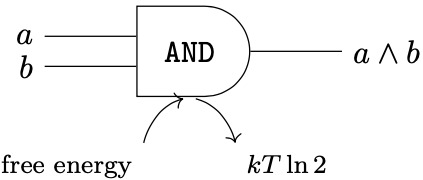
\includegraphics[width=5cm]{assets/and.png}
\end{center}
It is logically irreversible since the output does not allow for a complete reconstruction of the input. A way to make a computation logically reversible would be to use a \textbf{history tape} to a Turing Machine for storing the entire path of the computation. This solution, though, is not sustainable. This is because the original state of the history tape is lost and replaced by the waste piled up.

\begin{center}
	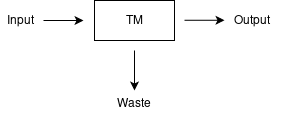
\includegraphics[width=5cm]{assets/irreversible_tm.png}
\end{center}
Bennett's idea was to eliminate the waste in an \textit{orderly fashion}. This means that the waste was \textbf{uncomputed} instead of erased. Here the output of the computation is copied onto some extra bit positions, and then the computation is undone step by step in reverse order.

\begin{center}
	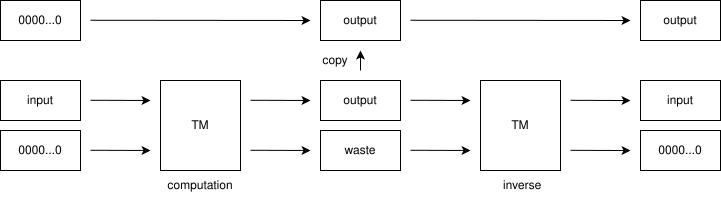
\includegraphics[width=12cm]{assets/reversible_tm.png}
\end{center}
We have seen that any computation can now be made logically reversible. Furthermore, \textbf{Friedkin} and \textbf{Toffoli} demonstrated that every logically reversible computation could be carried out in a thermodynamically reversible way. This was shown with the elastic collision of balls onto a billiard table. Loss of information is impossible due to the time-reversal symmetry of the laws of classical mechanics.

\subsection{Toffoli Gate}
The Toffoli gate is a made-reversible \textbf{AND} gate. This is done by adding an output wire for each input wire. This makes sure that the output of the gate contains the input values of the gate. This is the schematic for the \textbf{Toffoli Gate}:

\begin{center}
	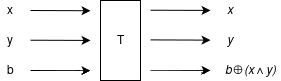
\includegraphics[width=7cm]{assets/toffoli.png}
\end{center}
The Toffoli gate is \textbf{universal}. This means that any circuit can be translated into a Toffoli gate. This follows from the possibility to get -- from one Toffoli gate each -- the \textbf{NOT}, \textbf{AND}, and \textbf{FAN-OUT}.

\begin{center}
	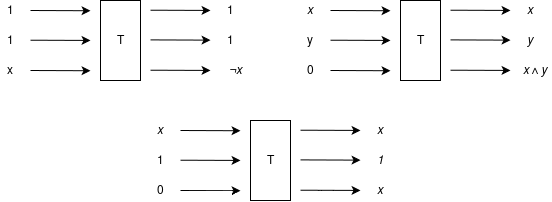
\includegraphics[width=12cm]{assets/not_and_fanout.png}
\end{center}
To remove the \textbf{junk} from a circuit, we can now use the following two gates:

\begin{center}
	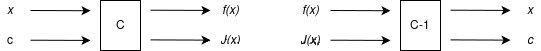
\includegraphics[width=11cm]{assets/junk.png}
\end{center}
Bennett's trick to uncompute the junk is the following:

\begin{enumerate}
	\item Apply $C$
	\item The output we want is copied using the Toffoli gate
	\item Use $C^{-1}$ to uncompute the junk
\end{enumerate}
The following is the visual representation of such circuit:

\begin{center}
	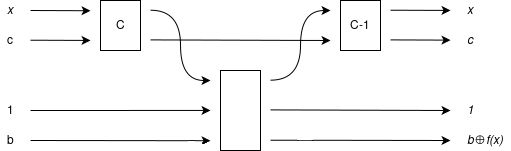
\includegraphics[width=11cm]{assets/remove_junk.png}
\end{center}
From this, we can conclude that the best reversible circuit is half as efficient as its irreversible counterpart.

\section{Key Experiments and Postulates of Quantum Physics}
The \textbf{UV catastrophe of black body radiation} and the \textbf{photoelectric effect} lead to the development of quantum physiscs.

\subsection{Black-Body Radiation}
\subsubsection{Classical Mechanics}
In classical statistical mechanics, the \textbf{law of equipartition} expresses the idea that, in thermal equilibrium, energy is usually shared over all possible corresponding microstates. If we assume the head to be transferred by electromagnetic waves, the equipartition law leads to problematic consequences. \\ \\
Let's imagine the following, we have a \textbf{cubic vacuum} with side length $l$. This vacuum has the following properties:

\begin{itemize}
	\item It absorbs and emits all radiation frequencies
	\item It is in thermodynamic equilibrium with its environment, in a heat bath of temperature $T$
\end{itemize}

\begin{center}
	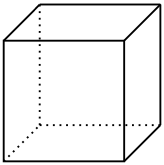
\includegraphics[width=2cm]{assets/cube.png}
\end{center}
The thermal electromagnetic radiation within this body can be thought of as \textbf{standing waves} within the body. Generally, a \textbf{standing wave} is a superposition of three standing waves, each corresponding to one spacial direction. Thus, a wave can be described by a three-dimensional vector of positive integers
\[ \overrightarrow n = (n_1, n_2, n_3) \in (\mathbb{N}_{> 0})^3 \]

\begin{center}
	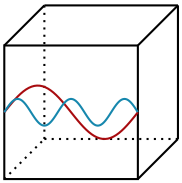
\includegraphics[width=2cm]{assets/standing_waves.png}
\end{center}
If we consider a shell of radius $|\overrightarrow n|$, then the number of waves scales with the scaling of the shell. This means that the number of waves also becomes $|\overrightarrow n|^2$. Likewise, the energy density scales with the square of the frequency
\[ \omega = c \pi \displaystyle\frac{|\overrightarrow n|}{l} \]
This growth in energy is referred to as \textbf{ultraviolet catastrophe}. This is absurd since, for instance, if we take a classroom at room temperature, everyone in it would drop dead immediately due to the intensity of the X-rays. \\ \\
For lower frequencies of waves, the quadratic dependence of the spectral radiance on the frequency matches experimental findings -- the \textbf{Rayleigh-Jeans Law}. In the case of higher frequencies, the spectral radiance exponentially decreases again.

\begin{center}
	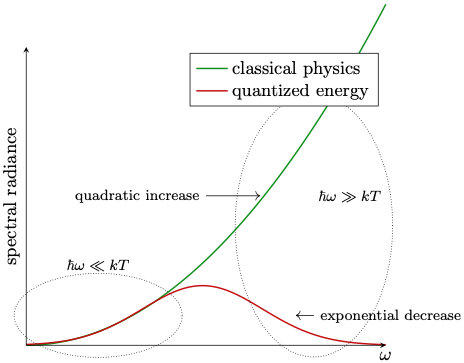
\includegraphics[width=6cm]{assets/spectral_radiance.png}
\end{center}
\subsubsection{Quantum Mechanics}
Max Plank discovered that the probability of emission and absorption of the cube would exponentially decrease at higher frequencies. He assumed that the radiation energy to be absorbed and emitted multiplies $\hbar \omega$, where $\hbar = 1.054 \times 10^{-34}Nms$. The probability of emission or absorption decreases exponentially in
\[ \frac{\hbar \omega}{kT} \]
In particular, the probability falls off exponentially for higher frequencies.

\subsection{Photoelectric Effect}
\subsubsection{Classical Mechanics}
By examining the emission of electrons from a metal surface if a light is shone onto it, the expectation was that the velocity of the emitted electrons faster depends on the intensity of the light but is independent of the frequency of the light --  i.e., its color. \\ \\
However, from experimental findings, Hertz found out that the intensity of the light merely changed the number of electrons. By increasing the frequency of the light, the velocity of the electrons increased. Below a specific frequency $\omega_0$, there were no emitted electrons, whatever the intensity or the duration of shining the light onto the surface.

\begin{center}
	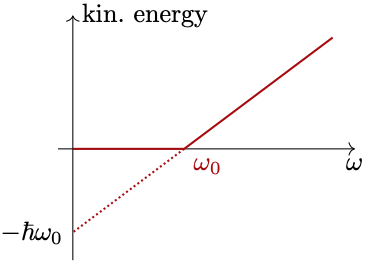
\includegraphics[width=4cm]{assets/photoelectric.png}
\end{center}

\subsubsection{Quantum Mechanics}
Alber Einstein explained the behavior observed by Plank. Einstein regarded light as a quantized packet of a certain frequency-dependent energy. Light comes in packets of $\hbar \omega$ energy. If the frequency is lower than $\omega_0$, then the energy lies below the energy $W = \hbar\omega_0$ needed to remove the electrons from the metal. Thus, the kinetic energy of the electron becomes
\[ E_{kin} = \hbar \omega - W \]
This shows the fundamental dualism in quantum mechanics, the \textbf{wave-particle dualism}.

\subsection{Wave-Particle Dualism}
We now examine the wave-particle dualism by using the example of a plane wave:
\[ \psi(\overrightarrow x, t) = C \cdot e^{i(\overrightarrow k \cdot \overrightarrow x - \omega t)} \]
Where $\overrightarrow k$ is the \textbf{wave vector} -- which is perpendicular to the wavefront. The relation between the wavelength and the wave vector is:
\[ \lambda = \frac{2\pi}{|\overrightarrow k|} \]
The \textbf{period} of the wave -- i.e., the time that elapses between the passage of two wavefronts -- is:
\[ \Delta t = \frac{2\pi}{\omega} \]
The \textbf{phase velocity} -- i.e., the velocity of the wavefront -- is:
\[ v = \frac{\omega}{|\overrightarrow k|} \]
If we examine the partial derivative of the plane wave, we obtain:
\[ \frac{\partial}{\partial t} \psi(\overrightarrow x, t) = - \frac{\hbar^2}{2m}\Delta\psi \]
Which directly corresponds to the \textbf{Shr\"odinger equation of a free particle}.
\[ i \hbar \frac{\partial}{\partial t} \psi = - \frac{\hbar^2}{2m}\Delta\psi \]

\subsubsection{Schr\"odinger's Equation}
The Sch\"odinger equation of a free particle has two fundamental properties:

\begin{itemize}
	\item \textbf{It is linear} \\
	Any linear combination of solution of the Schr\"odinger equation
	\[ \psi(\overrightarrow x, t) = \alpha\psi(\overrightarrow x, t) + \beta\psi(\overrightarrow x, t) ~~~~~~~~ \forall \alpha, \beta \in \mathbb{C}  \]
	Will again yield a solution.
	
	\item \textbf{It preserves the inner product} \\
	This means that a solution can be written as
	\[ \psi(\overrightarrow x, t) = U(t) \psi(\overrightarrow x, 0) \]
	Thus, the \textbf{time evolution operator} is unitary. This also implies that the \textbf{time evolution in quantum mechanics is reversible}.
\end{itemize}

\subsection{Postulates of Quantum Theory}
The postulates of quantum mechanics form the axiomatic basis of the theory.

\subsubsection{The State}
In quantum mechanics, a system (e.g. an electron, a photon, or an atom) is assigned a \textbf{normalized state vector} in a complex Hilbert space:
\[ \psi(\overrightarrow x, t) \in H ~~~~~~~~ \text{with}~||\psi|| = 1 \]

\subsubsection{The Time Evolution}
The time evolution of a quantum state is governed by the \textbf{Schr\"odinger equation}:
\[ \displaystyle\frac{\hbar}{i} \frac{\partial \psi}{\partial t} = H \psi \]

\subsubsection{The Observables}
In quantum mechanics, measurable entities correspond to observables. These are Hermitian operators $A$ with $A^\dagger = A$. More generally, \textbf{any Hermitian operator is an observable}. \\ \\
The \textbf{spectral theorem} for finite-dimensional linear operators states that an operator $A$ has a spectral decomposition with real eigenvalues if and only if the operator is Hermitian. Thus, an observable -- which is Hermitian by definition -- has a corresponding spectral decomposition. \\ \\
From the spectral decomposition, we obtain the weighted sum over all possible results of the measurement corresponding to $A$.

\subsubsection{Joint Systems and Composition}
Any linear combination in any of the subspaces corresponds to a linear combination in the joint space. This is an essential characteristic of the \textbf{tensor product}. Given two Hilbert spaces $H_A$ and $H_B$, the joint system has a state-space that is isomorphic to the tensor product of the Hilbert spaces -- $H_A \otimes H_B$. \\ \\
If the systems are in \textbf{pure states} $\psi_A \in H_A ~\text{and}~ \psi_B \in H_B$, then the joint state becomes:
\[ \psi_A \otimes \psi_B \in H_A \otimes H_B \]
However, any superposition of such product states is also a state in the joint Hilber space, and such superpositions may not have a representation as a product. Such states are said to be \textbf{entangled}.

\subsubsection{Astraction and Simplification}
If we assume the Hilbert space to be finite-dimensional, then this Hilbert space is isomorphic to an $n$ dimensional complex vector space $H \cong \mathbb{C}^n$. With this assumption, the states can be expressed by coordinates with respect to some fixed basis. \\ \\
For $\varphi \in H \cong \mathbb{C}^n$, we call the corresponding vector \textbf{ket} of $\varphi$, and represent it as:
\[ |\varphi\rangle = \begin{bmatrix} \varphi_1 \\ \varphi_2 \\ \vdots \\ \varphi_n \end{bmatrix} \]
Similarly, a \textbf{bra} is the conjugate transpose of a \textbf{ket}.
\[ \langle\varphi| = |\varphi\rangle^\dagger = \begin{bmatrix} \overline \varphi_1 & \overline \varphi_2 & \cdots & \overline \varphi_n \end{bmatrix} \]
Now, we can write the inner product as:
\[ (\varphi, \psi) = \begin{bmatrix} \overline \varphi_1 & \overline \varphi_2 & \cdots & \overline \varphi_n \end{bmatrix} \begin{bmatrix} \varphi_1 \\ \varphi_2 \\ \vdots \\ \varphi_n \end{bmatrix} = \langle \varphi|\psi\rangle \in \mathbb{C} \]
This is known as \textbf{Dirac's Bra-ket notation}. This notation is useful in expressing Hamiltonian observables. For example, the effect of an observable $A$ on a vector $\psi$, can be expressed as:
\[ |A\psi \rangle = \displaystyle \sum_i \lambda_i |P_{\varphi_i} \psi \rangle = \sum_i \lambda_i |\varphi_i \rangle \langle \varphi_i||\psi \rangle = \sum_i \lambda_i |\varphi_i \rangle \langle \varphi_i| \]
Where $|\varphi_i \rangle \langle \varphi_i|$ is the common way to represent a \textbf{projector}. A linear operator on a finite-dimensional vector space can be represented with a fixed basis as a matrix. In Dirac's notation, we can abbreviate the basis vector to their indices ($|\varphi_i \rangle =: |i\rangle$), this reads as:
\[ A = \displaystyle\sum_{k,l} \langle k | A | l \rangle |k\rangle \langle l| \]
Where $\langle k | A | l \rangle$ is the \textbf{matrix entry} of the $k$-th row and the $l$-th column. A property of the bra-ket notation is that:
\[ \sum_i |i\rangle\langle i| = \mymathbb{1} \]

\subsubsection{The Trace}
The trace is an important linear map $End(\mathcal{H}) \rightarrow \mathbb{C}$ defined as the sum over the diagonal elements of the matrix corresponding a linear operator $A \in End(\mathcal{H})$.
\[ Tr(A) := \sum_k \langle k|A|k\rangle \]

\subsubsection{Density Matrix}
A density matrix represents a statistical mixture of states. This matrix is defined as $\rho$ and is a positive trance-one operator. So $\rho$ is both Hermitian and all its eigenvalues are positive and sum to one.
\[ \rho = \sum_i \lambda_i |\varphi_i\rangle \langle \varphi_i| \]
\[ \sum_i \lambda_i = 1 \]
The eigenvalues can be regarded as probabilities for the system to be in the state of the corresponding eigenvector.

\subsubsection{The Time Evolution}
The time evolution of density matrices derives from the unitary propagator
\[ U(t) = e^{iHt/\hbar} \]
To be:
\[ \rho(t) = U(t)\rho(0)U^\dagger(t) \]

\subsubsection{The Probability}
The probability of obtaining the result $\lambda_i$ when measuring an observable $A$ is:
\[ P(\lambda_i) = Tr(|\varphi_i\rangle \langle\varphi_i|\rho) \]
Where $\varphi_i$ is the \textbf{eigenvector} corresponding to the eigenvalue $\lambda_i$ of $A$.

\subsubsection{Pure States}
The density matrices with no uncertainties -- which are those with eigenvalues corresponding to a deterministic probability distribution -- are the \textbf{projectors} on $\mathcal{H}$.

\subsubsection{Separability and Entanglement}
States of a joint system $H_A \otimes H_B$ that can be written as a product
\[ \psi = \varphi_A \otimes \varphi_B \]
are called \textbf{separable}. On the other hand, states that are not separable are called \textbf{entangled}. Let's consider the entangled \textbf{singlet} state:
\[ | \psi^- \rangle = \displaystyle\frac{1}{\sqrt{2}} (| 1 \rangle_B - | 1 \rangle_A \otimes | 0 \rangle_B) \]
This state is a \textbf{superposition} of pure states, thus a pure state itself. On the contrary, density matrices are convex combinations of \textbf{projectors} -- unless we are dealing with the special case of a pure density matrix.

\subsection{CNOT Gate}
The CNOT gate can be seen as a made-reversible XOR. The schematics for such a gate is:
\begin{center}
	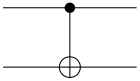
\includegraphics[width=2cm]{assets/cnot.png}
\end{center}
The CNOT can generate \textbf{entanglement}:
\begin{center}
	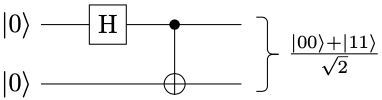
\includegraphics[width=5cm]{assets/entanglement.png}
\end{center}
This combination between the Hadamard gate (which puts the input in superposition) and the CNOT (which, combined with the Hadamard, generates an entangled state) is a change of basis between the standard basis and the \textbf{Bell basis}. The Bell basis is the following:
\[ \{ |\Phi^+\rangle, |\Phi^-\rangle, |\Psi^+\rangle, |\Psi^-\rangle \} \]
In particular, the following is a \textbf{Bell measurement}:
\begin{center}
	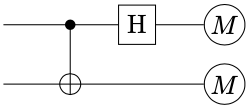
\includegraphics[width=3.5cm]{assets/bell_measurement.png}
\end{center}

\subsection{Cloning, Pseudo-Cloning, and Pseudo-Measurements}
To copy classical bits, we can use the CNOT gate. If the source is 0, then the CNOT gate does the following:
\begin{center}
	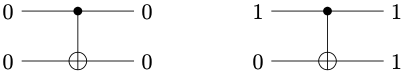
\includegraphics[width=6.5cm]{assets/cloning.png}
\end{center}
In the case of CNOT gates with $|0\rangle$ as a source, we can see that it also allows for \textbf{cloning} quantum information.
\begin{center}
	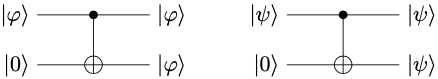
\includegraphics[width=6.5cm]{assets/cloning_2.png}
\end{center}
Only \textbf{parallel} and \textbf{orthogonal} states can be cloned by the CNOT. The cloning operation is not unitary, hence not allowed by quantum theory. This is known as the \textbf{no-cloning theorem}. The CNOT does not clone quantum states; it generates superpositions. This is why the action of the CNOT is sometimes referred to as \textbf{pseudo-cloning}. \\ \\
The CNOT can also be seen as a \textbf{pseudo-measurement} since there is no outcome. Moreover, because it is reversible, the CNOT is an \textbf{involution} -- i.e., a self inverse.

\section{Quantum Communication}
\subsection{Teleportation}
An object is said to be teleported from point $A$ to point $B$ if it is first at $A$ and at the end at $B$. However, the object must have never been anywhere in between $A$ and $B$. Moreover, the transfer does not have to be instantaneous -- as this would contradict relativity. \\ \\
Teleportation allows for carrying over the ability to transmit quantum information between two parties to a later point in time -- when only a classical channel is available. A priori, sending an unknown quantum state over a classical channel is \textbf{impossible}. If, however, the parties additionally both share entanglement, then it \textbf{becomes possible}.
\begin{center}
	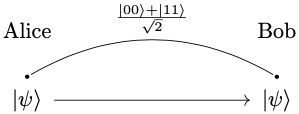
\includegraphics[width=4cm]{assets/teleportation.png}
\end{center}

\pagebreak
\subsubsection{Circuit}
The teleportation circuit is the following:
\begin{center}
	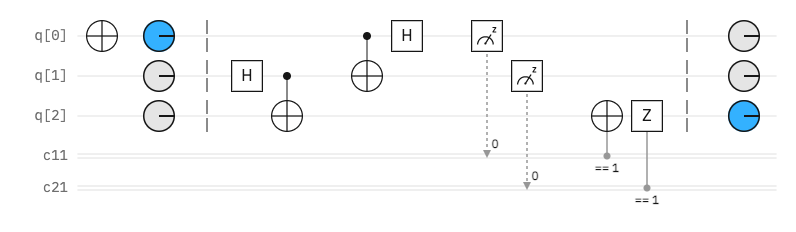
\includegraphics[width=11cm]{assets/teleportation_circuit.png}
\end{center}
As we can see from the diagram above, the Qbit $|1\rangle$ at state \verb|q[0]| -- which represents $|\varphi\rangle$ (i.e., the Qbit that Alice needs to send to Bob) -- has been teleported to \verb|q[2]| -- which represents Bob. \\ \\
In the \textbf{first step} of the circuit -- Hadamard + CNOT -- an entangled pair of Qbits is created and given to Alice (\verb|q[1]|) and Bob (\verb|q[2]|). In the \textbf{second step} of the circuit -- CNOT + Hadamard -- we prepare for a Bell measurement, which is done in \textbf{step three}. The two measurements are saved to two classical registers -- \verb|c11| and \verb|c21|. In \textbf{step four}, the final step, Bob now measures the bits sent by Alice. Bob, to read them, applies the transformation
\[ X^{b_1}Z^{b_2} \]
Where $X$ is a \textbf{X-pauli gate} (i.e., a negation), $Z$ is a \textbf{Z-Pauli gate} (i.e., a conditional phase flip), $b_1$ is the \textbf{bit on the} \verb|c21| \textbf{classical register} (sent to Bob by Alice), and $b_2$ is the \textbf{bit on the} \verb|c11| \textbf{classical register}. The transformations will only occur if the classical bit is equal to 1 (as we can see in the circuit above).

\subsubsection{Quantum Repeaters}
The main application of teleportation are \textbf{quantum repeaters}, which allow something called \textbf{entanglement-swapping}. There exist some device-independent cryptographic protocols. For these protocols, no trust in manufacturers and no correctness of quantum theory are required. \\ \\
The protocols are based on the parties sharing maximally entangled states. Such entanglement is complicated to establish over long distances. This is because the further the particles are transported, the more likely it is that they interact with the environment, thus losing their initial entanglement. \\ \\
If Alice and Bob are too far away from each other, we can use Charlie -- who is in between them -- to establish a \textbf{singlet} with both Alice and Bob. A property of teleportation is that if part of the entangled state is sent, then this entanglement is preserved. Charlie acts as a \textbf{quantum repeater}. \\ \\
In this cryptographic context, a downside of the \textbf{quantum repeater} is that the inner node -- i.e., the repeater -- must be trusted.

\subsection{Superdense Coding}
The scenario of superdense coding is the exact opposite of that of teleportation. In the case of teleportation, we use two classical bits to transport one Qbit. On the other hand, in the case of superdense coding, we transmit two bits using one Qbit. \\ \\
The circuit is the following:
\begin{center}
	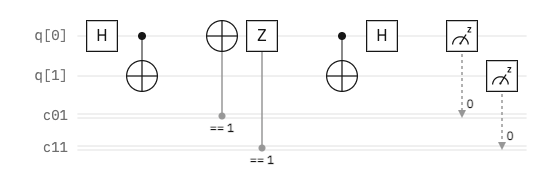
\includegraphics[width=8cm]{assets/superdense_circuit.png}
\end{center}
In the \textbf{first step} of the circuit -- Hadamard + CNOT -- an entangled pair of Qbits is created and given to Alice (\verb|q[1]|) and Bob (\verb|q[2]|). In the \textbf{second step} -- X-Pauli + Z-Pauli -- we encode the two classical bits. To encode these bits we use the following transformation:
\[ X^{b_1}Z^{b_2} \]
Where $b_1$ and $b_2$ are the \textbf{classical bits}. This transformation is the same as the one done in the teleportation. We prepare for a Bell measurement in the \textbf{third step} of the circuit -- CNOT + Hadamard. In \textbf{step four}, the final step, we perform the measurement -- i.e., decoding the originally sent bits.

\section{Simple Algorithms}
\subsection{$n$ Qbits}
The state space of systems of $n$ Qbits is the $n$-fold tensor product of $\mathbb{C}^2$ with itself:
\[ \mathcal{H} = \mathbb{C}^2 \otimes \mathbb{C}^2 \otimes \dots \otimes \mathbb{C}^2 \equiv \mathbb{C}^{2^n} \]
A basis of the space is given by the classical basis characterized through the set of all \textbf{classical} $n$-bit strings:
\[ \{ |i\rangle~|~i \in \{ 0, 1 \}^n \} \]
The action of the $n$-fold, bitwise, \textbf{Hadamard transform} is:
\[ H^{\otimes n} |i\rangle = \displaystyle\bigotimes^n_{l = 1} \left( \frac{|0\rangle + (-1)^{i_1} |1\rangle}{\sqrt{2}} \right) = \frac{1}{2^{n/2}} \displaystyle\sum_{j \in \{ 0,1 \}^n} (-1)^{i \cdot j}|j\rangle \]
Where the product $i \cdot j$ is defined as:
\[ i \cdot j := \displaystyle\bigotimes^n_{k=1} = i_k \wedge j_k \]
The product is always 0 if \textbf{one} of the two strings is the all-zero string 0. This means that the Hadamard applied to this vector has only plus signs. \textbf{This is the equal superposition of all classical states and will be the input for all quantum algorithms}. This is known as \textbf{quantum parallelism}. The state $|0\rangle$ also always has a positive sign.

\subsection{The Secret Mask}
Let $s \in \{ 0,1 \}^n$. Then $f_s$ is the function from $n$ bits to 1 bit:
\[ f_s := s \cdot x = \displaystyle\bigotimes^n_{i=1}(s_i \wedge x_i) \]
To find out $s$, one must make exactly $n$ queries. This algorithm is \textbf{optimal}, and only one bit of information per query is learned. The above function is for classical circuits; this cannot be directly translated to a quantum circuit. This is because classical circuits are \textbf{non-reversible}. Thus we need another function $\tilde f_s$, that is reversible:
\[ \tilde f_s (x, b) = (x, b \oplus f_s(x)) \]
This reversible function can now be represented as a reversible quantum circuit:
\begin{center}
	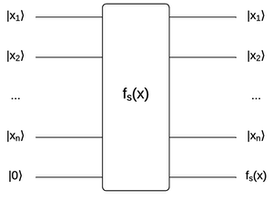
\includegraphics[width=5cm]{assets/circuit1.png}
\end{center}
It can be queried with the equal superpositions of classical inputs. This can be obtained by applying an Hadamard gate to each input wire -- except the last one.
\begin{center}
	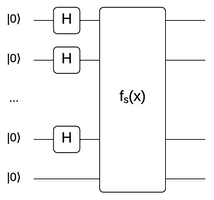
\includegraphics[width=4cm]{assets/circuit2.png}
\end{center}
The joint input of the output wires is now:
\[ \displaystyle\frac{1}{2^{n/2}} \sum_j (|j\rangle \otimes |f_s(j)\rangle) \]
This is \textbf{quantum parallelism}. This means that a single execution of the circuit allows for generating a state containing the function value for all inputs simultaneously. Though, such parallelism alone is not very helpful. \\ \\
To improve the circuit, let's add a Hadamard to the last wire:
\begin{center}
	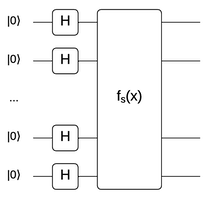
\includegraphics[width=4cm]{assets/circuit3.png}
\end{center}
Now the circuit acts as the identity and thus cannot be of any help. For this reason we flip the last state from $|0\rangle$ to $|1\rangle$. By doing so, the addition of the mapping becomes a subtraction, which is not commutative. The circuit becomes:
\begin{center}
	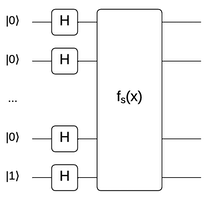
\includegraphics[width=4cm]{assets/circuit4.png}
\end{center}
For the given function, the sign factor equals to $(-1)^{j\cdot s}$, and all the $n$ Qbits are in the state $H^{\otimes n}|s\rangle$. Thus, if we apply $H$ again, this will yield $|s\rangle$ on the first $n$ Qbits.
\begin{center}
	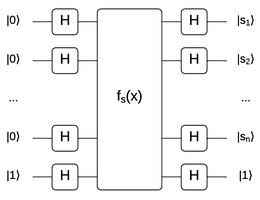
\includegraphics[width=5cm]{assets/circuit5.png}
\end{center}
The initial problem can be solved with one single call to the above quantum circuit. This algorithm combines the following two tricks:
\begin{enumerate}
	\item \textbf{Quantum Parallelism}
	\item \textbf{Phase Kick-back} \\
	When the state input on the result wire is $H|1\rangle$, then the function's output is encoded in a phase factor of the state of the input wires.
\end{enumerate}
	
\subsection{Deutsch/Josza Algorithm}
Let
\[ f~:~\{ 0, 1 \}^n \rightarrow \{ 0, 1 \} \]
Together with the promise that $f$ is either \textbf{constant} -- i.e., $f \equiv 0$ or $f \equiv 1$, or \textbf{balanced} -- i.e., $|\{ x|f(x) = 0 \}| = |\{ x|f(x) = 1 \}| = 2^{n-1}$ The circuit needs to decide whether $f$ is \textbf{constant} or \textbf{balanced}. Given a classical circuit, the number of calls would be in the order of:
\[ \displaystyle\frac{2^n}{2} + 1 \]
In the case of the quantum circuit, we would need only 1 call. The quantum circuit is the following:
\begin{center}
	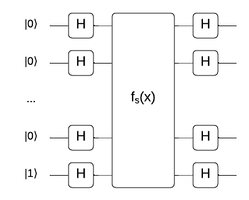
\includegraphics[width=5cm]{assets/circuit6.png}
\end{center}
The state after the first Hadamard gate is:
\[ \displaystyle\frac{1}{2^{n/2}} \sum_j |j\rangle \otimes H|1\rangle \]
The state, after the $f$-gate, then becomes:
\[ \displaystyle\frac{1}{2^{n/2}} \sum_j (-1)^{f(j)} |j\rangle \otimes H|1\rangle \]
The final $n$-fold Hadamard gate is applied to this state. The probability amplitude of only the output state $|000\dots 0\rangle$ is equal to:
\begin{itemize}
	\item 0 - if $f$ is \textbf{balanced}
	\item 1 - if $f \equiv 0$ -- i.e., \textbf{constant}
	\item -1 - if $f \equiv 1$ -- i.e., \textbf{constant}
\end{itemize}
This means that the output is \textbf{always} measured when $f$ is \textbf{constant}, but \textbf{never} when the function is \textbf{balanced}.























\pagebreak
\section{Glossary}
\subsection{Magnetic Dipole Moment}
The magnetic dipole moment is a vector that represents the strength and orientation of a magnet or other object that produces a magnetic field (e.g., an electron).

\subsection{Singlet}
A singlet is a maximally-entangled state. However, this one has nicer transformation properties differently from other maximally-entangled states. For instance, a singlet written with respect to a general basis has the same form as the standard basis.

\subsection{Hilbert Spaces}
The Hilbert spaces are the state spaces of quantum-mechanical systems. Quantum informatics happens in finite-dimensional Hilbert spaces -- while, in general, they can be infinite-dimensional. \\ \\
For a given dimension, there exists \textbf{exactly one} Hilbert space.

\subsection{Hermitian Operator}
A linear operator is said to be self-adjoint or Hermitian if and only if
\[ A^\dagger = A \]

\subsection{Unitary Operator}
A linear operator is said to be unitary if and only if
\[ U \cdot U^\dagger = 1 \]

\subsection{Superposition}
Any convex combination of state vectors:
\[ \alpha \psi_1 + \beta \psi_2 \in H ~~~~~~~~ \alpha, \beta \in \mathbb{C}~\text{with}~ |\alpha|^2 + |\beta|^2 = 1 \]
Is again a vector associated with a state of the system. Correspondingly, this linear structure of the state space gives rise to the interference effects and, generally, the wave characteristics of quantum mechanics.

\end{document}
